\documentclass{standalone}
\usepackage{tikz}
\usetikzlibrary{patterns, positioning}
\usepackage[sfdefault]{ClearSans} %% option 'sfdefault' activates Clear Sans as the default text font
\usepackage[T1]{fontenc}

\begin{document}
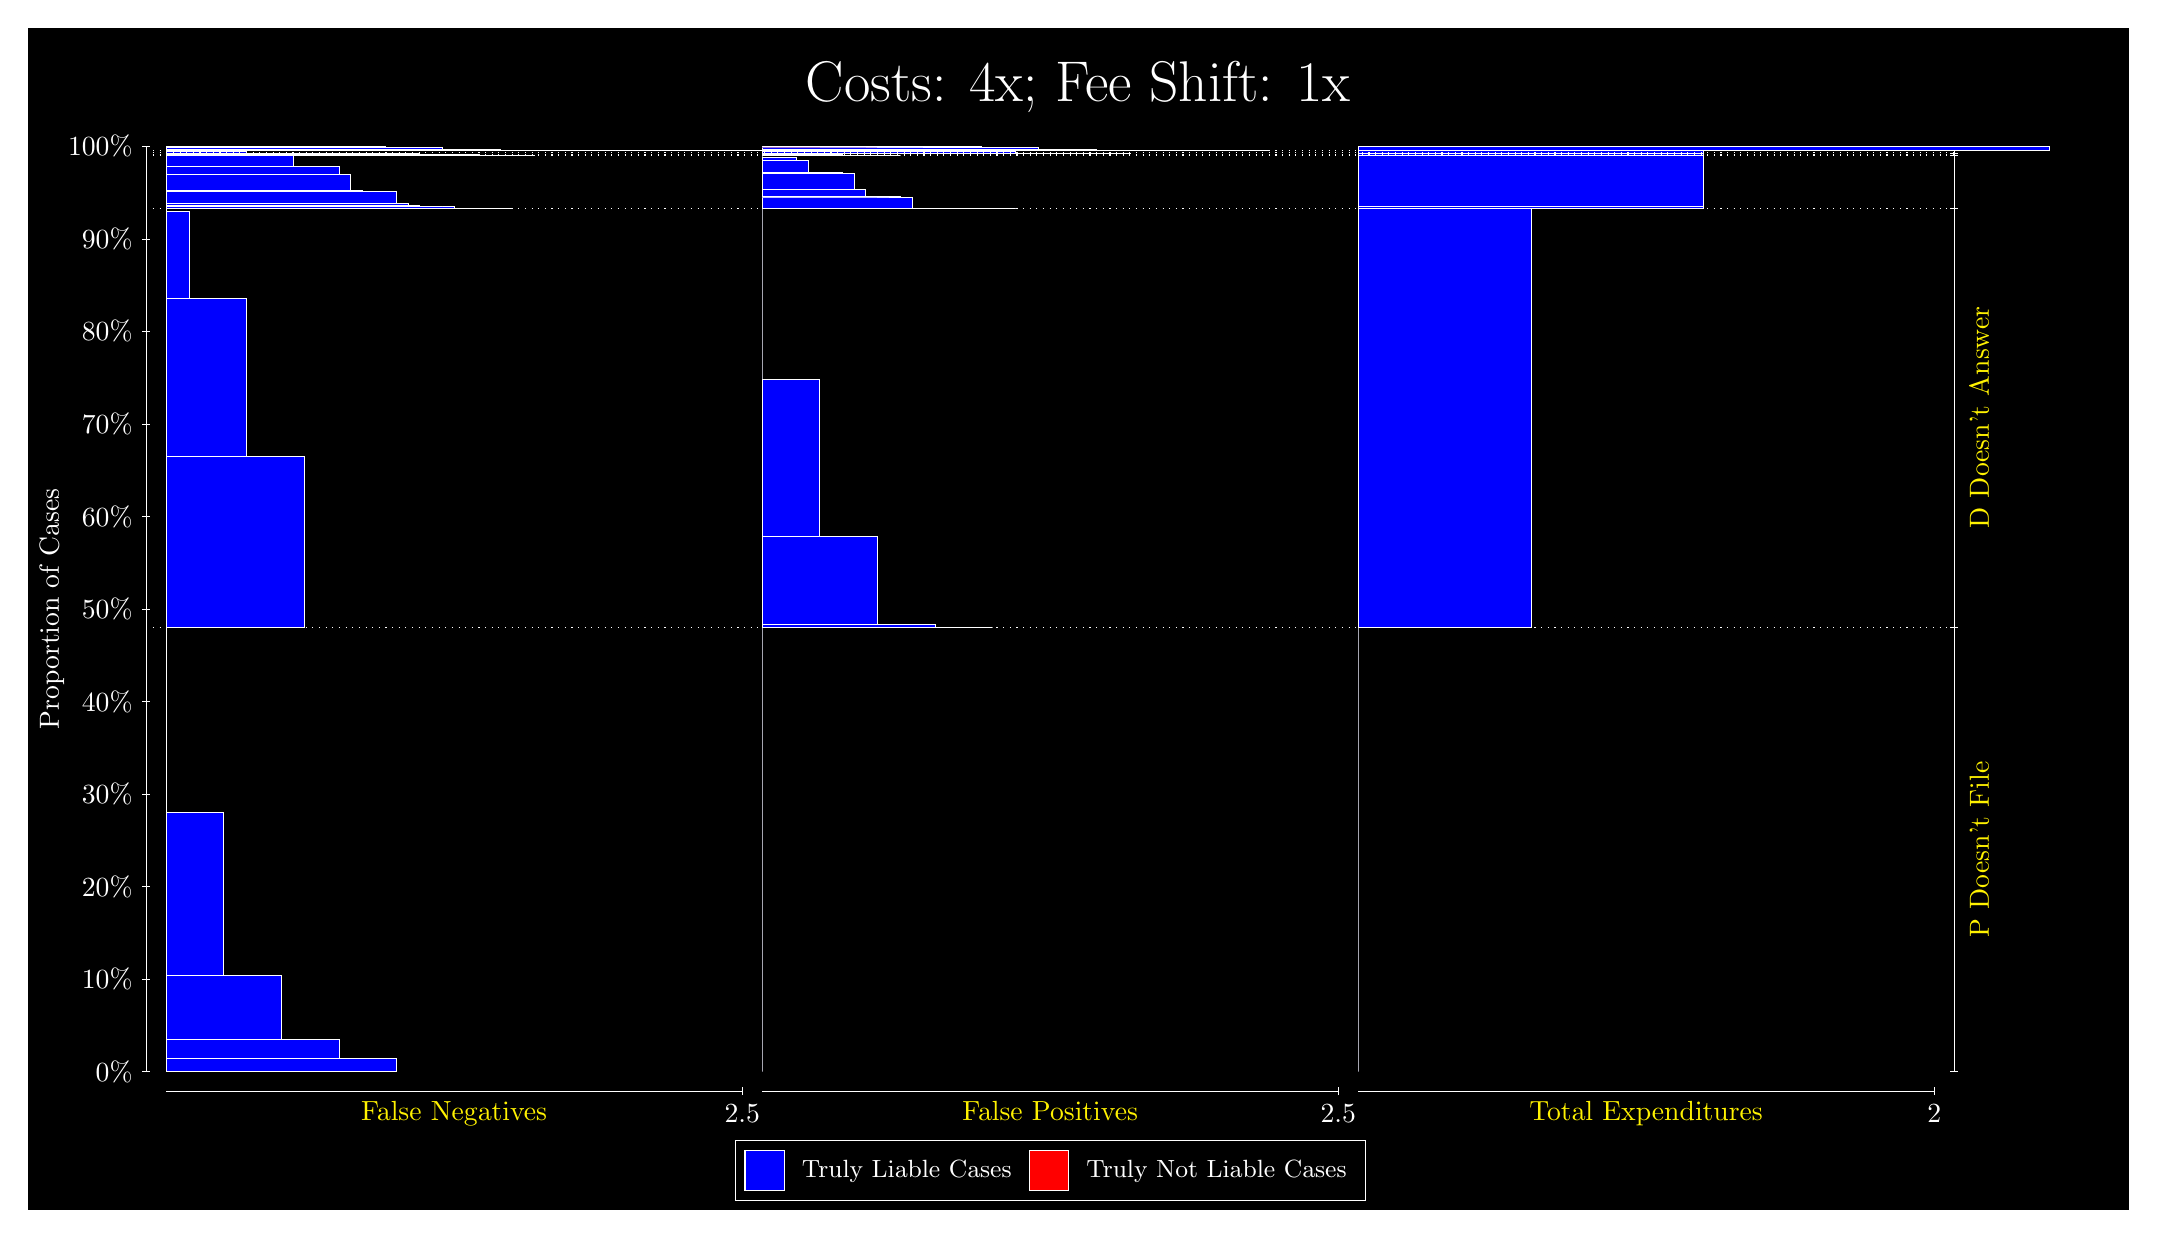
\begin{tikzpicture}
\draw[fill=black] (0,0) rectangle (26.667,15);
\draw[text=white] (0,13.5) rectangle (26.667,15) node[midway] {\huge Costs: 4x; Fee Shift: 1x};
\draw[white, very thin] (1.5,1.75) -- (1.5,13.5);
\node[rotate=90, text=white, anchor=center] at (0.3, 7.625) {Proportion of Cases};
\draw[white, very thin] (1.45,1.75) -- (1.55,1.75);
\node[text=white, anchor=east] at (1.45, 1.75) {0\%};
\draw[white, very thin] (1.45,2.925) -- (1.55,2.925);
\node[text=white, anchor=east] at (1.45, 2.925) {10\%};
\draw[white, very thin] (1.45,4.1) -- (1.55,4.1);
\node[text=white, anchor=east] at (1.45, 4.1) {20\%};
\draw[white, very thin] (1.45,5.275) -- (1.55,5.275);
\node[text=white, anchor=east] at (1.45, 5.275) {30\%};
\draw[white, very thin] (1.45,6.45) -- (1.55,6.45);
\node[text=white, anchor=east] at (1.45, 6.45) {40\%};
\draw[white, very thin] (1.45,7.625) -- (1.55,7.625);
\node[text=white, anchor=east] at (1.45, 7.625) {50\%};
\draw[white, very thin] (1.45,8.8) -- (1.55,8.8);
\node[text=white, anchor=east] at (1.45, 8.8) {60\%};
\draw[white, very thin] (1.45,9.975) -- (1.55,9.975);
\node[text=white, anchor=east] at (1.45, 9.975) {70\%};
\draw[white, very thin] (1.45,11.15) -- (1.55,11.15);
\node[text=white, anchor=east] at (1.45, 11.15) {80\%};
\draw[white, very thin] (1.45,12.325) -- (1.55,12.325);
\node[text=white, anchor=east] at (1.45, 12.325) {90\%};
\draw[white, very thin] (1.45,13.5) -- (1.55,13.5);
\node[text=white, anchor=east] at (1.45, 13.5) {100\%};

\draw[white, very thin] (24.457,1.75) -- (24.457,13.5);
\draw[white, very thin] (24.407,1.75) -- (24.507,1.75);
\node[anchor=west] at (24.407, 1.75) {};
\draw[white, very thin] (24.407,7.3941) -- (24.507,7.3941);
\node[anchor=west] at (24.407, 7.3941) {};
\draw[white, very thin] (24.407,12.716) -- (24.507,12.716);
\node[anchor=west] at (24.407, 12.716) {};
\draw[white, very thin] (24.407,13.39) -- (24.507,13.39);
\node[anchor=west] at (24.407, 13.39) {};
\draw[white, very thin] (24.407,13.416) -- (24.507,13.416);
\node[anchor=west] at (24.407, 13.416) {};
\draw[white, very thin] (24.407,13.452) -- (24.507,13.452);
\node[anchor=west] at (24.407, 13.452) {};
\draw[white, very thin] (24.407,13.5) -- (24.507,13.5);
\node[anchor=west] at (24.407, 13.5) {};

\draw[white, very thin, fill=blue] (1.75,1.75) rectangle (4.6775,1.9186);
\draw[white, very thin, fill=blue] (1.75,1.9186) rectangle (3.9457,2.1589);
\draw[white, very thin, fill=blue] (1.75,2.1589) rectangle (3.2138,2.9741);
\draw[white, very thin, fill=blue] (1.75,2.9741) rectangle (2.4819,5.0469);
\draw[white, very thin, fill=red] (1.75,5.0469) rectangle (1.75,5.0469);
\draw[white, very thin, fill=blue] (1.75,5.0469) rectangle (1.75,7.3941);
\draw[white, very thin, fill=blue] (1.75,7.3941) rectangle (3.5065,9.5673);
\draw[white, very thin, fill=blue] (1.75,9.5673) rectangle (2.7746,11.564);
\draw[white, very thin, fill=blue] (1.75,11.564) rectangle (2.0428,12.678);
\draw[white, very thin, fill=red] (1.75,12.678) rectangle (1.75,12.678);
\draw[white, very thin, fill=blue] (1.75,12.678) rectangle (1.75,12.716);
\draw[white, very thin, fill=blue] (1.75,12.716) rectangle (6.1413,12.716);
\draw[white, very thin, fill=blue] (1.75,12.716) rectangle (5.8486,12.716);
\draw[white, very thin, fill=blue] (1.75,12.716) rectangle (5.5558,12.717);
\draw[white, very thin, fill=blue] (1.75,12.717) rectangle (5.4094,12.743);
\draw[white, very thin, fill=blue] (1.75,12.743) rectangle (5.2631,12.743);
\draw[white, very thin, fill=blue] (1.75,12.743) rectangle (5.1167,12.744);
\draw[white, very thin, fill=blue] (1.75,12.744) rectangle (4.9703,12.75);
\draw[white, very thin, fill=blue] (1.75,12.75) rectangle (4.8239,12.782);
\draw[white, very thin, fill=blue] (1.75,12.782) rectangle (4.6775,12.93);
\draw[white, very thin, fill=blue] (1.75,12.93) rectangle (4.5312,12.931);
\draw[white, very thin, fill=blue] (1.75,12.931) rectangle (4.3848,12.933);
\draw[white, very thin, fill=blue] (1.75,12.933) rectangle (4.2384,12.946);
\draw[white, very thin, fill=blue] (1.75,12.946) rectangle (4.092,13.15);
\draw[white, very thin, fill=blue] (1.75,13.15) rectangle (3.9457,13.246);
\draw[white, very thin, fill=blue] (1.75,13.246) rectangle (3.7993,13.246);
\draw[white, very thin, fill=blue] (1.75,13.246) rectangle (3.6529,13.247);
\draw[white, very thin, fill=blue] (1.75,13.247) rectangle (3.5065,13.25);
\draw[white, very thin, fill=blue] (1.75,13.25) rectangle (3.3602,13.387);
\draw[white, very thin, fill=blue] (1.75,13.387) rectangle (3.2138,13.388);
\draw[white, very thin, fill=blue] (1.75,13.388) rectangle (3.0674,13.388);
\draw[white, very thin, fill=blue] (1.75,13.388) rectangle (2.921,13.388);
\draw[white, very thin, fill=blue] (1.75,13.388) rectangle (2.7746,13.388);
\draw[white, very thin, fill=blue] (1.75,13.388) rectangle (2.6283,13.39);
\draw[white, very thin, fill=blue] (1.75,13.39) rectangle (2.3355,13.39);
\draw[white, very thin, fill=blue] (1.75,13.39) rectangle (2.0428,13.39);
\draw[white, very thin, fill=red] (1.75,13.39) rectangle (1.75,13.39);
\draw[white, very thin, fill=blue] (1.75,13.39) rectangle (6.4341,13.39);
\draw[white, very thin, fill=blue] (1.75,13.39) rectangle (5.7022,13.398);
\draw[white, very thin, fill=blue] (1.75,13.398) rectangle (4.9703,13.412);
\draw[white, very thin, fill=blue] (1.75,13.412) rectangle (4.2384,13.416);
\draw[white, very thin, fill=blue] (1.75,13.416) rectangle (3.5065,13.416);
\draw[white, very thin, fill=red] (1.75,13.416) rectangle (1.75,13.416);
\draw[white, very thin, fill=blue] (1.75,13.416) rectangle (3.5065,13.416);
\draw[white, very thin, fill=blue] (1.75,13.416) rectangle (2.7746,13.437);
\draw[white, very thin, fill=blue] (1.75,13.437) rectangle (2.0428,13.452);
\draw[white, very thin, fill=red] (1.75,13.452) rectangle (1.75,13.452);
\draw[white, very thin, fill=blue] (1.75,13.452) rectangle (1.75,13.452);
\draw[white, very thin, fill=blue] (1.75,13.452) rectangle (11.704,13.452);
\draw[white, very thin, fill=blue] (1.75,13.452) rectangle (10.972,13.452);
\draw[white, very thin, fill=blue] (1.75,13.452) rectangle (10.24,13.453);
\draw[white, very thin, fill=blue] (1.75,13.453) rectangle (9.508,13.455);
\draw[white, very thin, fill=blue] (1.75,13.455) rectangle (8.7761,13.456);
\draw[white, very thin, fill=blue] (1.75,13.456) rectangle (8.0442,13.456);
\draw[white, very thin, fill=blue] (1.75,13.456) rectangle (7.4587,13.456);
\draw[white, very thin, fill=blue] (1.75,13.456) rectangle (7.3123,13.456);
\draw[white, very thin, fill=blue] (1.75,13.456) rectangle (6.7268,13.456);
\draw[white, very thin, fill=blue] (1.75,13.456) rectangle (5.9949,13.464);
\draw[white, very thin, fill=blue] (1.75,13.464) rectangle (5.2631,13.488);
\draw[white, very thin, fill=blue] (1.75,13.488) rectangle (4.5312,13.499);
\draw[white, very thin, fill=blue] (1.75,13.499) rectangle (3.7993,13.5);
\draw[white, very thin, fill=blue] (1.75,13.5) rectangle (3.0674,13.5);
\draw[white, very thin, fill=blue] (1.75,13.5) rectangle (2.3355,13.5);
\draw[white, very thin, fill=red] (1.75,13.5) rectangle (1.75,13.5);
\draw[white, very thin, fill=red] (9.3189,1.75) rectangle (9.3189,1.75);
\draw[white, very thin, fill=blue] (9.3189,1.75) rectangle (9.3189,7.3941);
\draw[white, very thin, fill=red] (9.3189,7.3941) rectangle (12.246,7.3941);
\draw[white, very thin, fill=blue] (9.3189,7.3941) rectangle (12.246,7.3941);
\draw[white, very thin, fill=blue] (9.3189,7.3941) rectangle (11.515,7.4322);
\draw[white, very thin, fill=blue] (9.3189,7.4322) rectangle (10.783,8.546);
\draw[white, very thin, fill=blue] (9.3189,8.546) rectangle (10.051,10.543);
\draw[white, very thin, fill=blue] (9.3189,10.543) rectangle (9.3189,12.716);
\draw[white, very thin, fill=red] (9.3189,12.716) rectangle (12.539,12.716);
\draw[white, very thin, fill=blue] (9.3189,12.716) rectangle (12.539,12.716);
\draw[white, very thin, fill=red] (9.3189,12.716) rectangle (12.246,12.716);
\draw[white, very thin, fill=blue] (9.3189,12.716) rectangle (12.246,12.716);
\draw[white, very thin, fill=red] (9.3189,12.716) rectangle (11.954,12.716);
\draw[white, very thin, fill=blue] (9.3189,12.716) rectangle (11.954,12.718);
\draw[white, very thin, fill=blue] (9.3189,12.718) rectangle (11.807,12.718);
\draw[white, very thin, fill=red] (9.3189,12.718) rectangle (11.661,12.718);
\draw[white, very thin, fill=blue] (9.3189,12.718) rectangle (11.661,12.718);
\draw[white, very thin, fill=blue] (9.3189,12.718) rectangle (11.515,12.718);
\draw[white, very thin, fill=red] (9.3189,12.718) rectangle (11.368,12.718);
\draw[white, very thin, fill=blue] (9.3189,12.718) rectangle (11.368,12.719);
\draw[white, very thin, fill=blue] (9.3189,12.719) rectangle (11.222,12.857);
\draw[white, very thin, fill=blue] (9.3189,12.857) rectangle (11.075,12.86);
\draw[white, very thin, fill=blue] (9.3189,12.86) rectangle (10.929,12.86);
\draw[white, very thin, fill=blue] (9.3189,12.86) rectangle (10.783,12.86);
\draw[white, very thin, fill=blue] (9.3189,12.86) rectangle (10.636,12.956);
\draw[white, very thin, fill=blue] (9.3189,12.956) rectangle (10.49,13.16);
\draw[white, very thin, fill=blue] (9.3189,13.16) rectangle (10.344,13.173);
\draw[white, very thin, fill=blue] (9.3189,13.173) rectangle (10.197,13.175);
\draw[white, very thin, fill=blue] (9.3189,13.175) rectangle (10.051,13.176);
\draw[white, very thin, fill=blue] (9.3189,13.176) rectangle (9.9044,13.324);
\draw[white, very thin, fill=blue] (9.3189,13.324) rectangle (9.758,13.356);
\draw[white, very thin, fill=blue] (9.3189,13.356) rectangle (9.6116,13.362);
\draw[white, very thin, fill=blue] (9.3189,13.362) rectangle (9.4652,13.363);
\draw[white, very thin, fill=blue] (9.3189,13.363) rectangle (9.3189,13.39);
\draw[white, very thin, fill=red] (9.3189,13.39) rectangle (11.075,13.39);
\draw[white, very thin, fill=blue] (9.3189,13.39) rectangle (11.075,13.39);
\draw[white, very thin, fill=blue] (9.3189,13.39) rectangle (10.344,13.394);
\draw[white, very thin, fill=blue] (9.3189,13.394) rectangle (9.6116,13.408);
\draw[white, very thin, fill=blue] (9.3189,13.408) rectangle (9.3189,13.416);
\draw[white, very thin, fill=red] (9.3189,13.416) rectangle (14.003,13.416);
\draw[white, very thin, fill=blue] (9.3189,13.416) rectangle (14.003,13.416);
\draw[white, very thin, fill=blue] (9.3189,13.416) rectangle (13.271,13.416);
\draw[white, very thin, fill=blue] (9.3189,13.416) rectangle (12.539,13.431);
\draw[white, very thin, fill=blue] (9.3189,13.431) rectangle (11.807,13.452);
\draw[white, very thin, fill=blue] (9.3189,13.452) rectangle (11.075,13.452);
\draw[white, very thin, fill=red] (9.3189,13.452) rectangle (15.759,13.452);
\draw[white, very thin, fill=blue] (9.3189,13.452) rectangle (15.759,13.452);
\draw[white, very thin, fill=blue] (9.3189,13.452) rectangle (15.028,13.452);
\draw[white, very thin, fill=red] (9.3189,13.452) rectangle (15.028,13.452);
\draw[white, very thin, fill=blue] (9.3189,13.452) rectangle (15.028,13.452);
\draw[white, very thin, fill=blue] (9.3189,13.452) rectangle (14.296,13.453);
\draw[white, very thin, fill=red] (9.3189,13.453) rectangle (14.296,13.453);
\draw[white, very thin, fill=blue] (9.3189,13.453) rectangle (14.296,13.453);
\draw[white, very thin, fill=blue] (9.3189,13.453) rectangle (13.564,13.456);
\draw[white, very thin, fill=red] (9.3189,13.456) rectangle (13.564,13.456);
\draw[white, very thin, fill=blue] (9.3189,13.456) rectangle (13.564,13.464);
\draw[white, very thin, fill=blue] (9.3189,13.464) rectangle (12.832,13.464);
\draw[white, very thin, fill=blue] (9.3189,13.464) rectangle (12.832,13.488);
\draw[white, very thin, fill=blue] (9.3189,13.488) rectangle (12.1,13.496);
\draw[white, very thin, fill=blue] (9.3189,13.496) rectangle (11.368,13.496);
\draw[white, very thin, fill=red] (9.3189,13.496) rectangle (10.783,13.496);
\draw[white, very thin, fill=blue] (9.3189,13.496) rectangle (10.783,13.496);
\draw[white, very thin, fill=blue] (9.3189,13.496) rectangle (10.636,13.496);
\draw[white, very thin, fill=red] (9.3189,13.496) rectangle (10.051,13.496);
\draw[white, very thin, fill=blue] (9.3189,13.496) rectangle (10.051,13.496);
\draw[white, very thin, fill=red] (9.3189,13.496) rectangle (9.3189,13.496);
\draw[white, very thin, fill=blue] (9.3189,13.496) rectangle (9.3189,13.5);
\draw[white, very thin, fill=red] (16.888,1.75) rectangle (16.888,1.75);
\draw[white, very thin, fill=blue] (16.888,1.75) rectangle (16.888,7.3941);
\draw[white, very thin, fill=red] (16.888,7.3941) rectangle (19.083,7.3941);
\draw[white, very thin, fill=blue] (16.888,7.3941) rectangle (19.083,12.716);
\draw[white, very thin, fill=red] (16.888,12.716) rectangle (21.279,12.716);
\draw[white, very thin, fill=blue] (16.888,12.716) rectangle (21.279,12.738);
\draw[white, very thin, fill=red] (16.888,12.738) rectangle (21.279,12.738);
\draw[white, very thin, fill=blue] (16.888,12.738) rectangle (21.279,13.39);
\draw[white, very thin, fill=red] (16.888,13.39) rectangle (21.279,13.39);
\draw[white, very thin, fill=blue] (16.888,13.39) rectangle (21.279,13.416);
\draw[white, very thin, fill=red] (16.888,13.416) rectangle (21.279,13.416);
\draw[white, very thin, fill=blue] (16.888,13.416) rectangle (21.279,13.452);
\draw[white, very thin, fill=red] (16.888,13.452) rectangle (25.67,13.452);
\draw[white, very thin, fill=blue] (16.888,13.452) rectangle (25.67,13.456);
\draw[white, very thin, fill=red] (16.888,13.456) rectangle (25.67,13.456);
\draw[white, very thin, fill=blue] (16.888,13.456) rectangle (25.67,13.5);
\draw[white, dotted] (1.5,7.3941) -- (24.457,7.3941);
\draw[white, dotted] (1.5,12.716) -- (24.457,12.716);
\draw[white, dotted] (1.5,13.39) -- (24.457,13.39);
\draw[white, dotted] (1.5,13.416) -- (24.457,13.416);
\draw[white, dotted] (1.5,13.452) -- (24.457,13.452);
\draw[white, very thin] (1.75,1.5) -- (9.0689,1.5);
\node[text=yellow, anchor=north] at (5.4094, 1.5) {False Negatives};
\draw[white, very thin] (9.0689,1.45) -- (9.0689,1.55);
\node[text=white, anchor=north] at (9.0689, 1.45) {2.5};

\draw[white, very thin] (9.3189,1.5) -- (16.638,1.5);
\node[text=yellow, anchor=north] at (12.978, 1.5) {False Positives};
\draw[white, very thin] (16.638,1.45) -- (16.638,1.55);
\node[text=white, anchor=north] at (16.638, 1.45) {2.5};

\draw[white, very thin] (16.888,1.5) -- (24.207,1.5);
\node[text=yellow, anchor=north] at (20.547, 1.5) {Total Expenditures};
\draw[white, very thin] (24.207,1.45) -- (24.207,1.55);
\node[text=white, anchor=north] at (24.207, 1.45) {2};

\node[text=yellow, centered, rotate=90] at (24.777, 4.5721) {P Doesn't File};
\node[text=yellow, centered, rotate=90] at (24.777, 10.055) {D Doesn't Answer};





\draw (12.978300999999998,1.5) node[draw=none] (baseCoordinate) {};
\begin{scope}[align=center]
        \matrix[scale=0.5, draw=white, below=0.5cm of baseCoordinate, nodes={draw}, column sep=0.1cm]{
            \node[rectangle, draw, minimum width=0.5cm, minimum height=0.5cm, fill=blue] {}; &
            \node[draw=none, font=\small, text=white] (B) {Truly Liable Cases}; &
            \node[rectangle, draw, minimum width=0.5cm, minimum height=0.5cm, fill=red] {}; &
            \node[draw=none, font=\small, text=white] (B) {Truly Not Liable Cases}; \\
            };
\end{scope}

\end{tikzpicture}
\end{document}